\chapter{Nuevos operadores para STL}
\label{cha:stl}

\section{Lógica Temporal}

Si navegamos por internet o buscamos en los libros acerca de qué es la lógica temporal tarde o temprano daremos con una cita del filósofo alemán Kant que cita: 

\begin{center}
\textit{``la posibilidad de principios apodícticos de las relaciones del tiempo, o axiomas del tiempo en general. Tiene una sola dimensión: los distintos tiempos no son simultáneos, sino sucesivos''}
\end{center}

Y, aunque quizás sacado de todo contexto, es un buen primer comienzo para explicar acerca de qué es el tiempo y por consiguiente qué tiene que ver la lógica con éste. Y es que Kant quería expresar que el tiempo es algo que va ocurriendo constantemente, es un conjunto de hechos que juntos transcurren en una dirección y conforman el tiempo. Pues bien, teniendo en cuenta esta idea podemos llegar a comprender y diferenciar la lógica temporal. 

La lógica proposicional no tiene la percepción de tiempo: en este tipo de lógica tenemos hechos que son verdaderos o falsos, que unidos pueden transformarse en verdad o no, pero nunca individualmente cambian su valor. Por ejemplo si decimos que:

\begin{center}
s = ``El día está soleado''
\end{center}

Este argumento será eterno individualmente. Aún así, realizamos operaciones con él como negarlo $\neg{s}$,: todo el argumento se verá afectado en todo momento.

\begin{center}
$\neg{s}$ = ``El día no está soleado''
\end{center}

Pero como todos podemos percibir, en la realidad esto no sucede. En otras palabras, puede que ``no todo el día esté soleado'', pero quizás si por la mañana y no por la tarde o viceversa. Esto es lo que trata de expresar la lógica temporal. En un momento determinado una expresión puede ser verdad mientras que en otra hora, minuto, segundo, o cualquier otra unidad que utilicemos para medir el tiempo, puede cambiar y tener un valor diferente. En un sistema ciberfísico, el controlador software se representa como una máquina de estados (Figura~\ref{fig:state_machine}).

\begin{figure}
\centering
  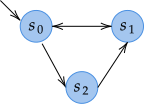
\includegraphics{images/state_machine}
\caption{Máquina de estados.}
\label{fig:state_machine}
\end{figure}

Tras el estado inicial $s_0$, la aplicación puede moverse de un estado a otro dependiendo de las restricciones de la máquina. Esto dará lugar a una traza de ejecución (Figura~\ref{fig:trace_discrete}) donde el \textit{tiempo} se refleja en el número de estados recorridos. En este ejemplo, el tiempo es \textit{discreto}: cada instante temporal está asociado a un único estado del sistema.

\begin{figure}
\centering
%  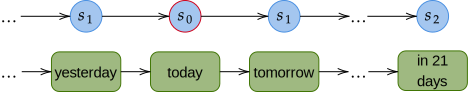
\includegraphics[width=.95\linewidth]{images/trace_discrete}
  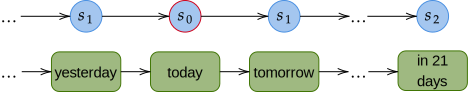
\includegraphics{images/trace_discrete}
\caption{Traza de ejecución (discreta).}
\label{fig:trace_discrete}
\end{figure}

En un entorno real, el tiempo es \textit{denso}, es decir, el estado de la aplicación cambia en función de los datos que registra en los sensores o en las reacciones que cambian un parámetro físico (Figura~\ref{fig:trace_dense}).

\begin{figure}
\centering
%  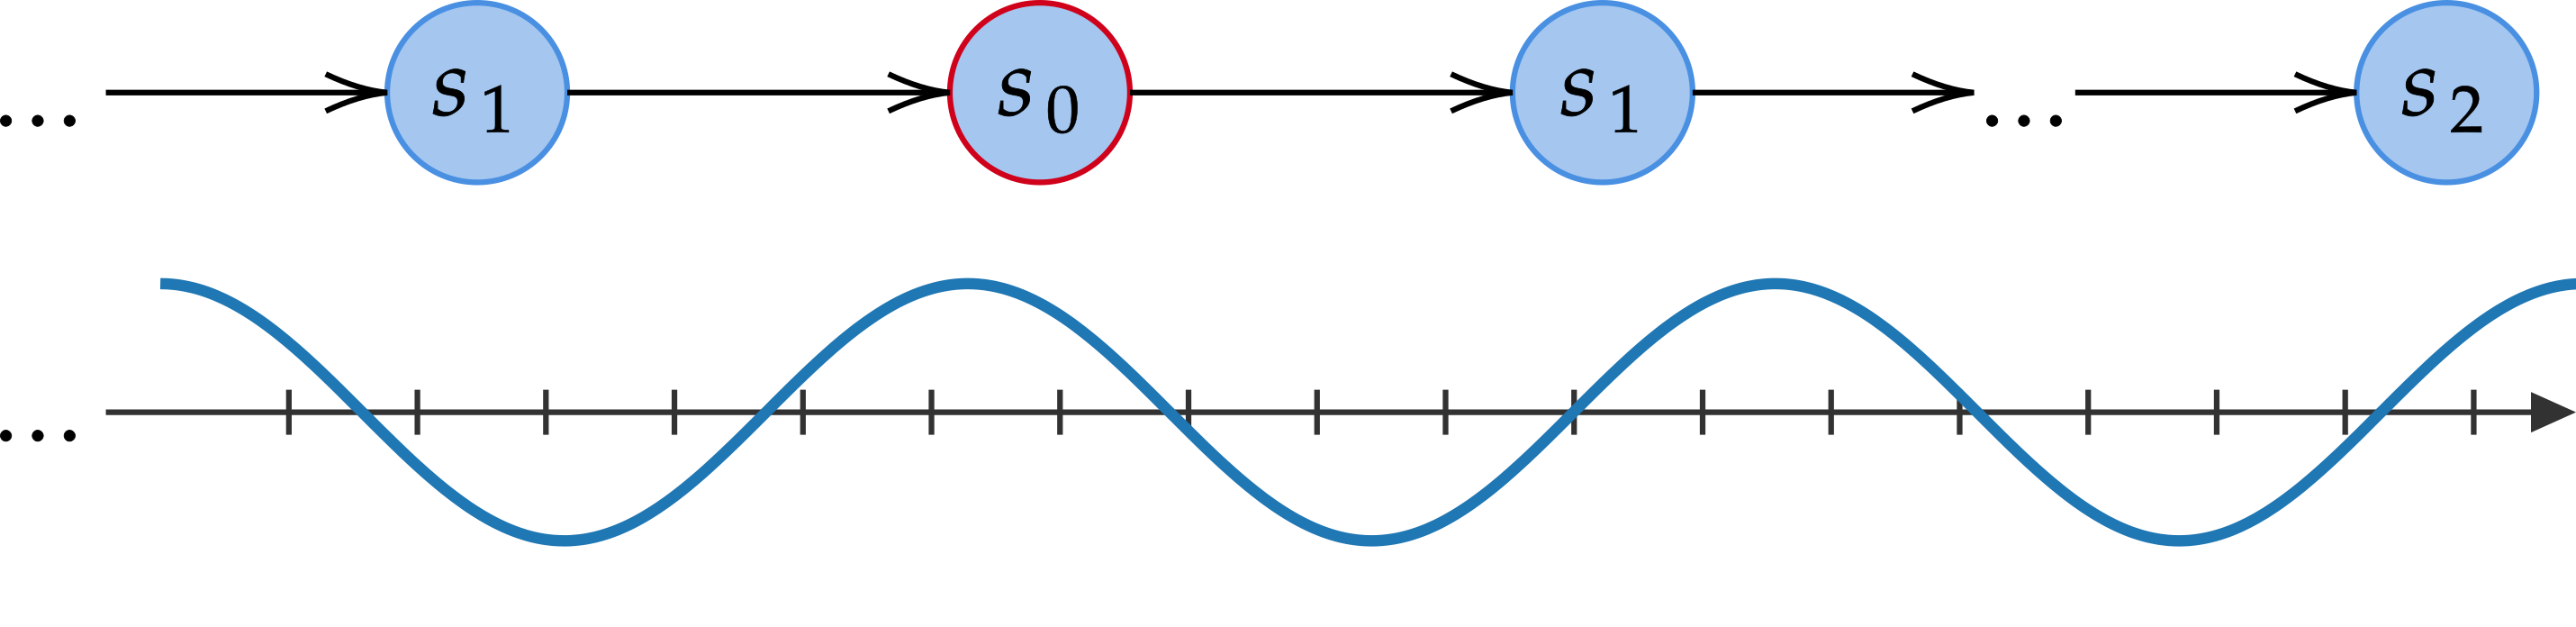
\includegraphics[width=.95\linewidth]{images/trace_dense}
  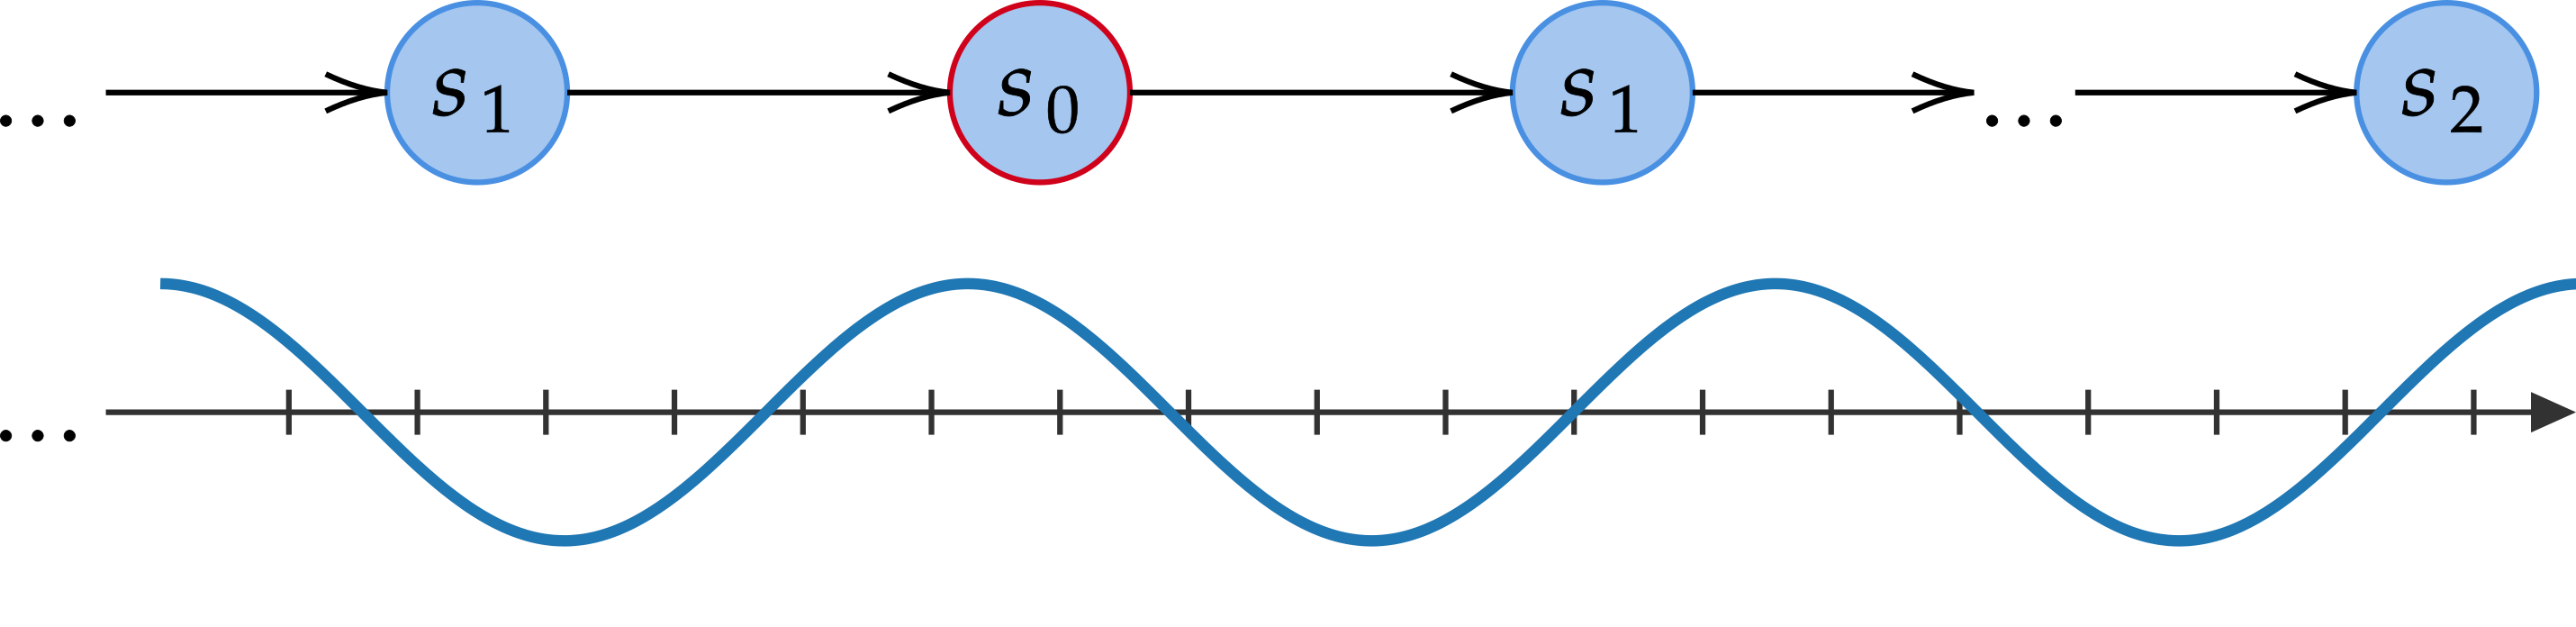
\includegraphics{images/trace_dense}
\caption{Traza de ejecución (densa).}
\label{fig:trace_dense}
\end{figure}

En este trabajo utilizaremos Signal Temporal Logic \cite{STL}, un tipo de lógica temporal enfocada al análisis de señales analógicas o reales.


\section{Signal Temporal Logic}
% Definición, sintaxis y semántica de los operadores.
\textit{Signal Temporal Logic} (STL) \cite{STL} es un tipo de lógica temporal especializada en el análisis de señales reales analógicas. STL permite expresar características sobre la evolución de algún atributo físico, como la velocidad o temperatura. Por tanto, como punto de partida, STL requiere una muestra o traza de ejecución sobre la que comprobar las hipótesis.

La lógica distingue dos tipos de situaciones: propiedades que se satisfacen en un \textit{estado} o momento puntual de la traza de ejecución, o propiedades de \textit{camino} que se evalúan a lo largo de una secuencia de eventos. STL proporciona operadores para recorrer los diferentes estados del sistema y comprobar en qué momentos se cumplen las propiedades.

Por ejemplo, la proposición atómica $v > 120$ mostraría los instantes en los que la velocidad supera los $120$. Los operadores de camino enriquecerían esa expresión para analizar si la velocidad se sobrepasa puntualmente en algún momento (\textbf{F})uturo del viaje, (\textbf{G})eneralmente a lo largo de todo el recorrido, o permanece constante hasta (\textbf{U}ntil) que se incrementa a un nuevo valor. 

Formalmente, la gramática básica de STL comprende los siguientes operadores:

$$ \varphi \ := \ \mu \ |\ \neg \varphi \ |\ \varphi_{1} \lor \varphi_{2} \ |\ \varphi_{1} U_{[t_1, t_2]} \varphi_{2}$$

Donde $\mu$ representa las proposiciones atómicas, en forma de desigualdades sobre la señal muestreada (p.ej., $\mu := v > 120$); y $\varphi$ las especificaciones sobre los caminos. El resto de los operadores se componen a partir de los operadores precedentes, donde $t_1, t_2 \in \mathbb{R}_{\geq 0}$ son marcas temporales que definen el intervalo de monitorización respecto al instante inicial, siendo $t_2 \geq t_1$. 

% Operador futuro y general

% $$ F_{[a,b]} \varphi \equiv \top U_{[a,b]} \varphi $$
% $$ G_{[a,b]} \varphi \equiv \neg F_{[a,b]} \neg \varphi $$

\begin{align*}
F_{[a,b]} \varphi \equiv \top U_{[a,b]} \varphi & &
G_{[a,b]} \varphi \equiv \neg F_{[a,b]} \neg \varphi
\end{align*}

Existen versiones extendidas que permiten analizar aspectos cuantitativas con STL, por ejemplo, los valores máximos/mínimos \cite{TACAS_19} o integrales en un intervalo, o calcular la derivada en un punto \cite{Stl_Der_Int}.


Las especificaciones en STL se \textit{compilan} en un monitor que supervisa la ejecución del sistema (p. ej., el sensor de velocidad de un vehículo). Algunos intérpretes de STL son AMT \cite{AMT2} (sintaxis básica) y STLEval \cite{StlEval} (sintaxis básica y operadores de min/max). En este proyecto, implementaremos en STLEval los operadores cuantitativos de STL que permiten calcular integrales y derivadas sobre una señal, según la definición propuesta en \cite{Stl_Der_Int}.

\section{STLEval}
%Lenguaje utilizado en STLEval (C++), etc.
STLEval es una herramienta capaz de manejar tanto expresiones STL básicas, que devuelven señales Booleanas, como ciertas extensiones cuantitativas, que transforman la señal de entrada en una nueva señal continua (operadores de min/max). Por estos motivos, así como su eficiencia (está escrita en en C++) STLEval se ha tomado como punto de partida para implementar los operadores cuantitativos de STL que permiten calcular integrales y derivadas sobre una señal, según la definición propuesta en \cite{Stl_Der_Int}.

% Muestreo de la señal. Representación interna en STLEval.
Internamente, STLEval representa una señal como una serie temporal, es decir, una sucesión de pares \textit{(clave, valor)} donde la \textit{clave} es una marca temporal y el \textit{valor} representa la magnitud física en ese momento. La imagen \ref{fig:senal} ilustra la señal original y su representación interna en STLEval. 

\begin{figure}
\centering
  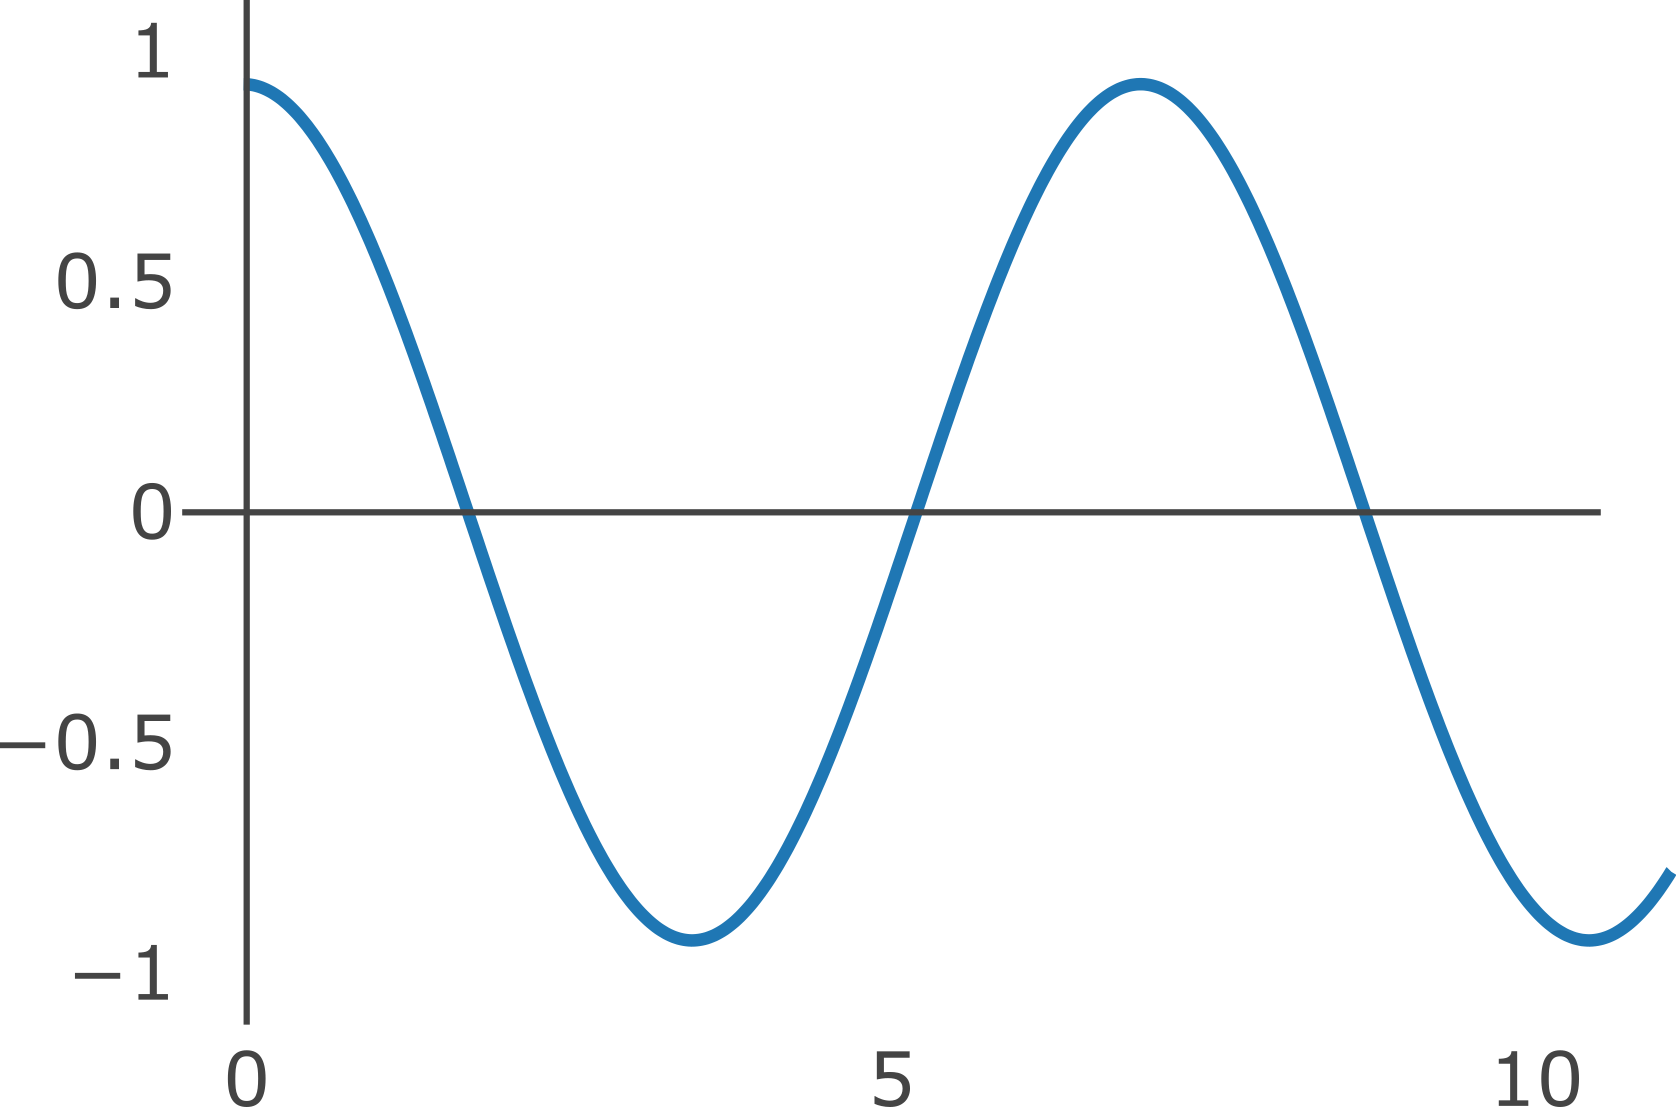
\includegraphics[width=.4\linewidth]{images/senal_original} \hfill
  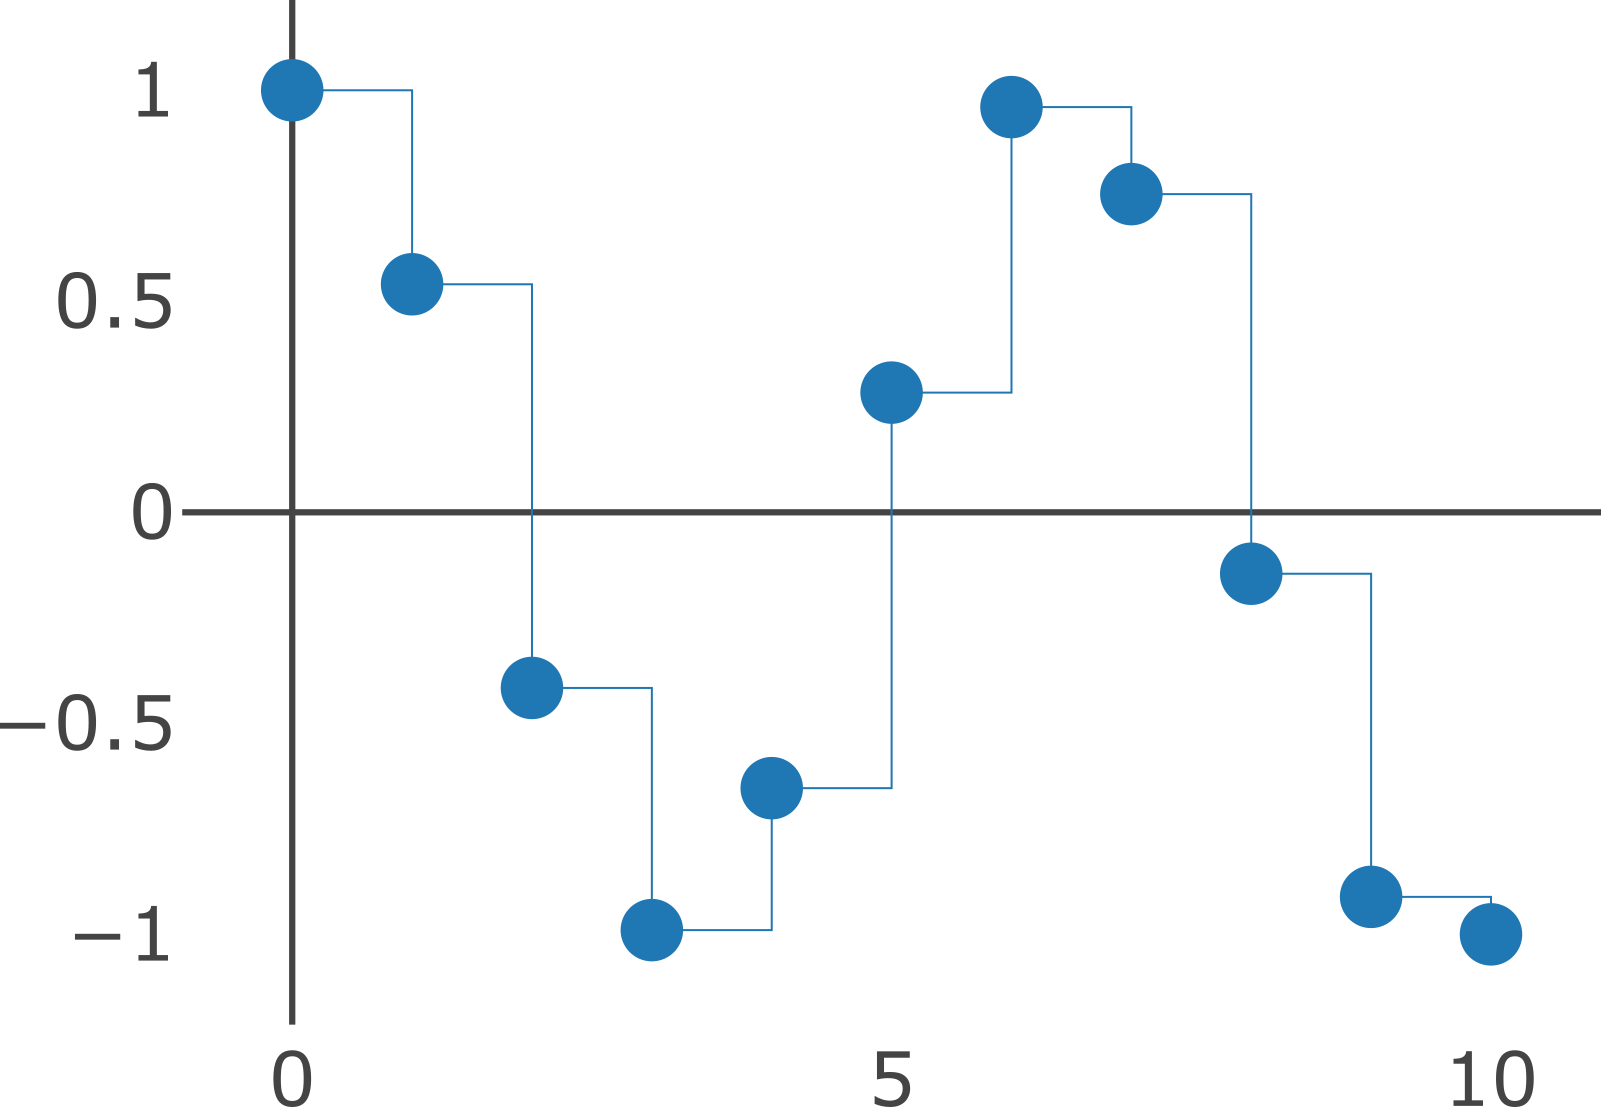
\includegraphics[width=.4\linewidth]{images/senal_muestreada}
\caption{Señal original y su reconstrucción.}
\label{fig:senal}
\end{figure}

\section{Definición de los nuevos operadores}

El cálculo de la derivada e integral se aproximan mediante las siguientes expresiones matemáticas, donde $\mathbf{x}$ representa la señal completa, $\mathbf{x}_{\tau}$ es el valor de la señal en el instante $\tau$, $\mu^i_{[a,b]}$ es la integral en el intervalo $[a, b]$ y $\mu^d_{+}$ ($\mu^d_{-}$) representan la aproximación de la derivada por la derecha (izquierda) del instante temporal en cuestión:

\begin{align*}
\mu^d_{+} &= \frac{dg(\mathbf{x})}{dt^+} \geq c & & \mu^i_{[a,b]} = \int^{b}_{a} g(\mathbf{x}_{\tau}) \delta \tau \geq c \\
\mu^d_{-} &= \frac{dg(\mathbf{x})}{dt^-} \geq c &
\end{align*}

Dado que internamente STLEval representa las señales reales como una serie numérica discreta, aproximamos el instante temporal $\tau$ como $\tau = k \delta t$ donde $\delta t$ es la frecuencia de muestreo y $k$ el término de la sucesión:

\begin{align*}
\mu^d_{+} &= g(\mathbf{x}_{(k + 1) \delta t}) - g(\mathbf{x}_{k \delta t}) \geq c \delta t & & \mu^i_{[a,b]} = \sum^{k + b / \delta t - 1}_{k' = k + a / \delta t} g(\mathbf{x}_{k' \delta t}) \delta t \geq c \\
\mu^d_{-} &= g(\mathbf{x}_{k \delta t}) - g(\mathbf{x}_{(k - 1) \delta t}) \geq c \delta t & 
\end{align*}

Gráficamente, la derivada se interpreta como la pendiente entre dos puntos consecutivos de la señal; y la integral como el sumatorio del área de los rectángulos con base  $\delta t$ contenidos en el intervalo (Figura \ref{fig:der_int}). 

\begin{figure}
\centering
  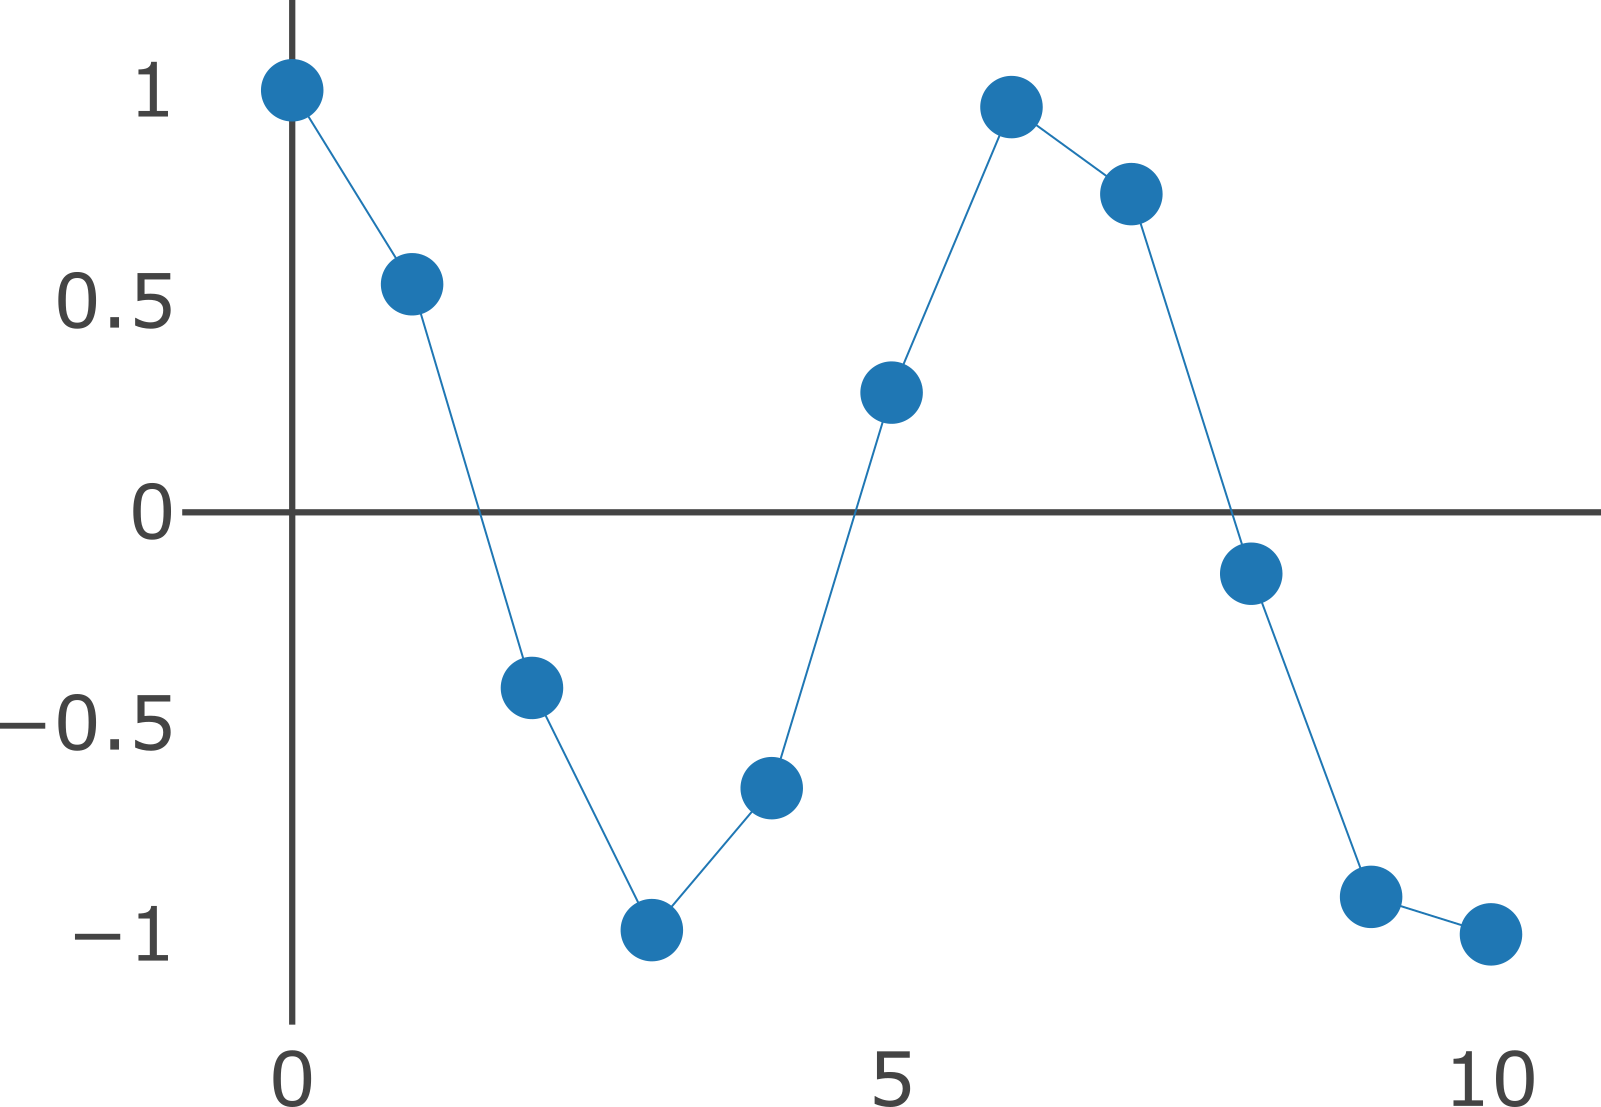
\includegraphics[width=.4\linewidth]{images/derivada} \hfill
  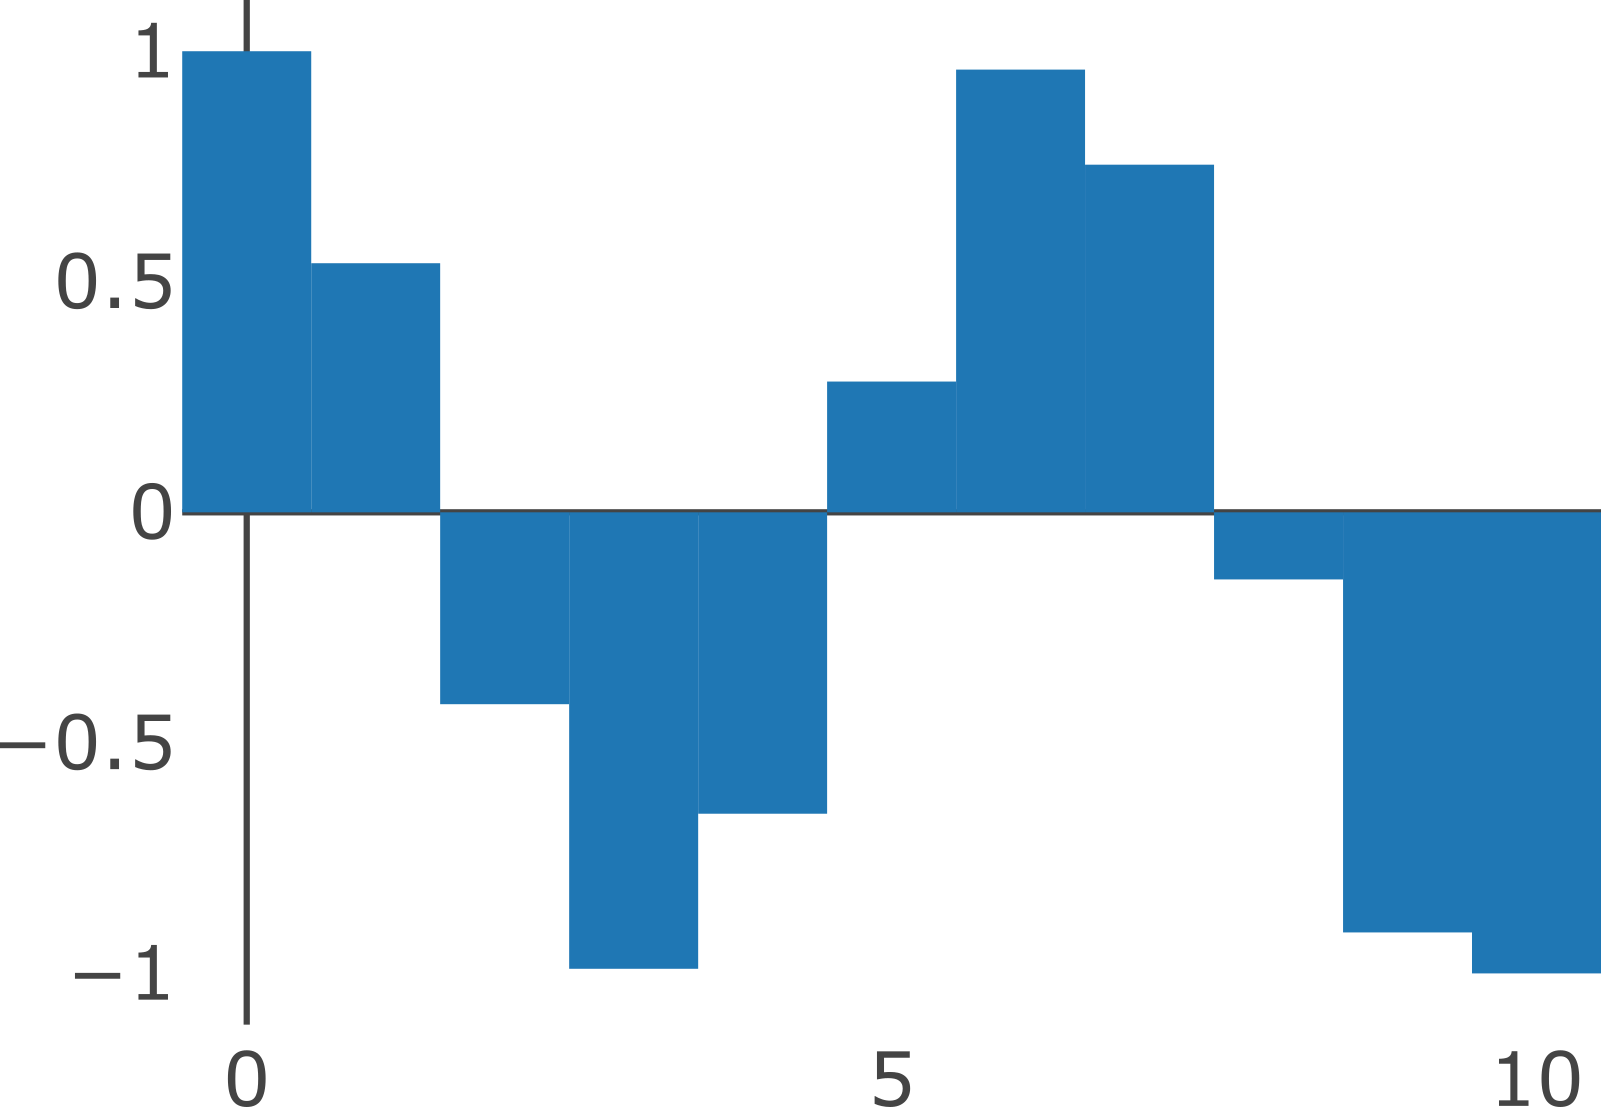
\includegraphics[width=.4\linewidth]{images/integral}
%  \includegraphics[width=.4\linewidth]{images/integral_old}
\caption{Interpretación de la derivada e integral.}
\label{fig:der_int}
\end{figure}

Los nuevos operadores se han incorporado a STLEval. En la notación de la herramienta, $D$ simboliza el operador derivada ($D \equiv \mu^d_{+}$), e $I$ representa el operador integral ($I_[a,b] \equiv \mu^i_{[a,b]}$).

\section{Integración con ParetoLib}
ParetoLib \cite{FORMATS_19, ParetoLib} es una biblioteca de minería que recibe una especificación paramétrica o plantilla en STL y devuelve el rango de valores de las variables para las que la propiedad se satisface o invalida. Internamente, ParetoLib implementa un algoritmo de búsqueda que guía el aprendizaje y evalúa instancias concretas de la fórmula temporal a través de la herramienta STLEval. Para ello, ParetoLib se empaqueta junto los binarios y librerías dinámicas de STLEval precompilados tanto para Linux como para Windows, lo que convierte a la biblioteca en una herramienta multiplataforma. 

\begin{figure}[htb]
\centering
  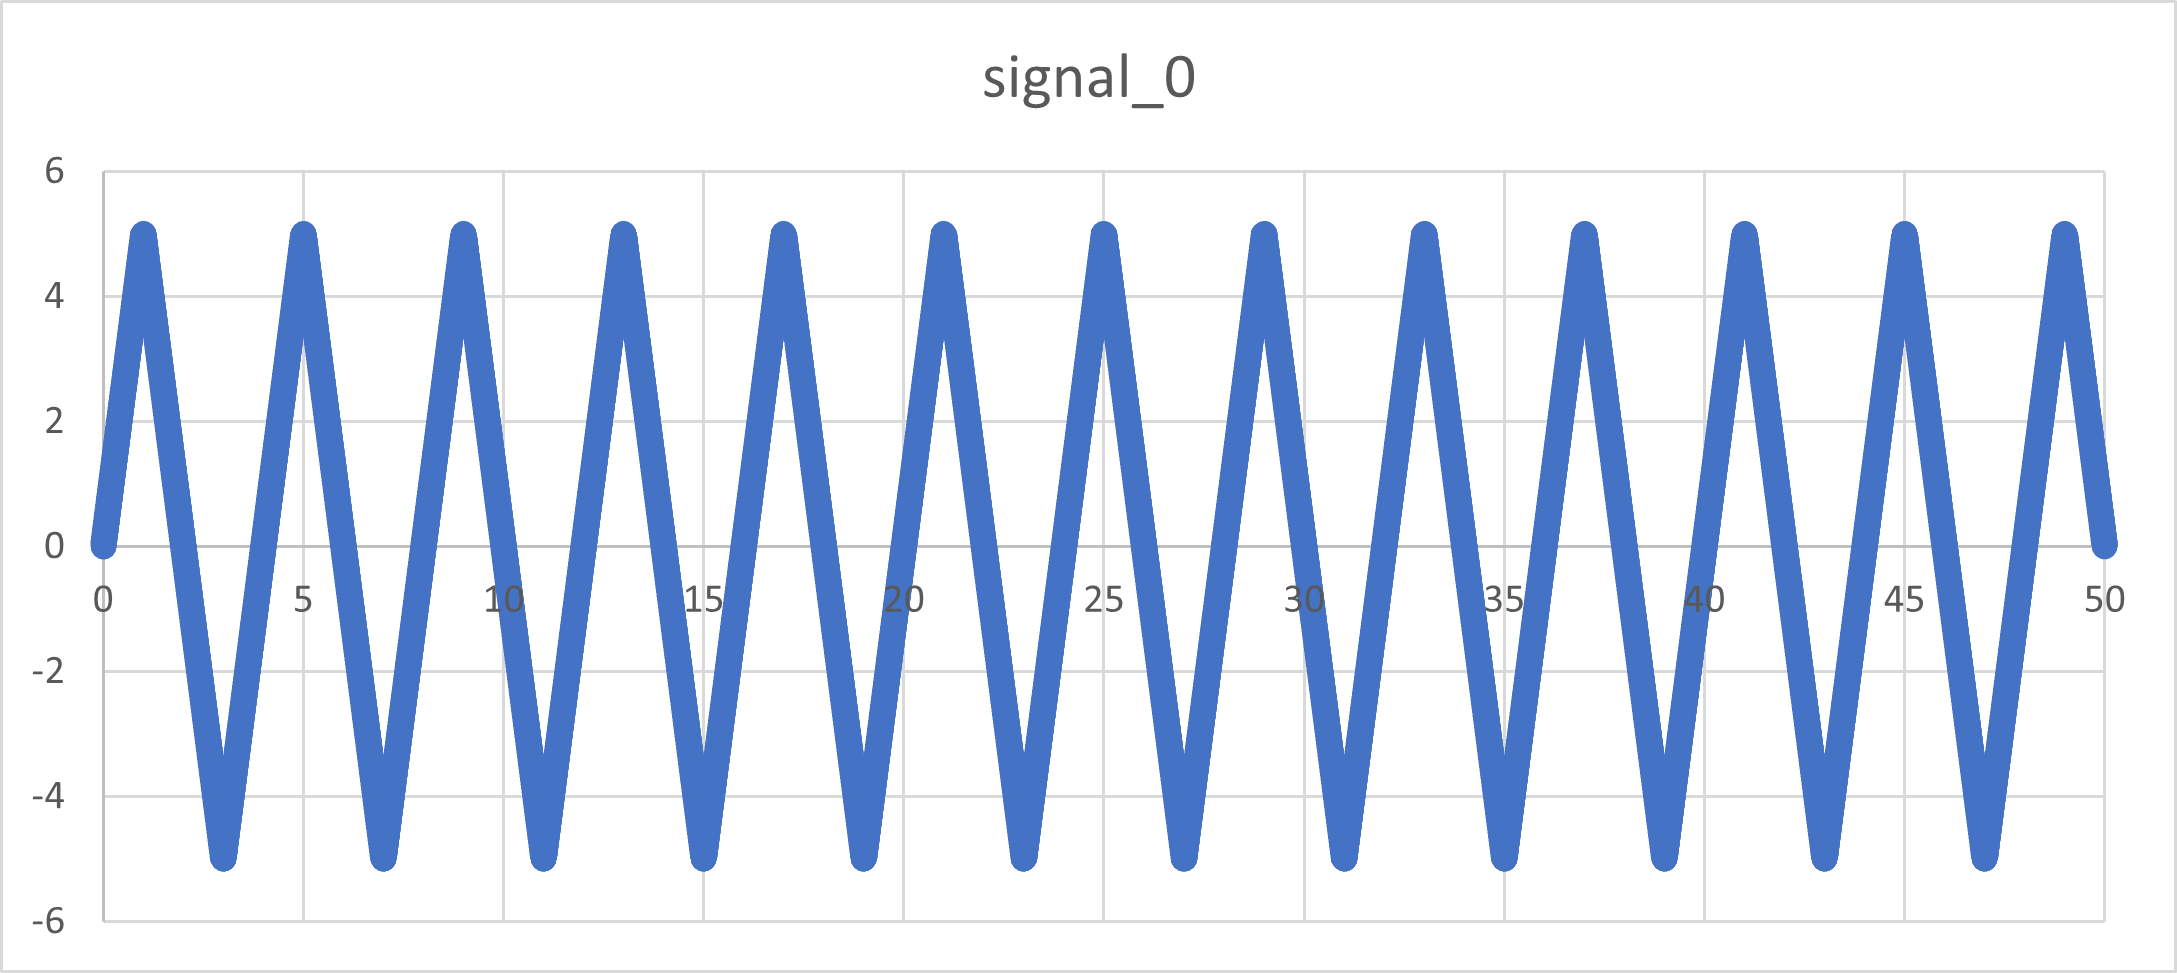
\includegraphics[width=0.7\linewidth]{images/triangular} 
\caption{Señal triangular.}
\label{fig:trian}
\end{figure}

Gracias a la actualización de STLEval, podemos evaluar expresiones que involucren parámetros en derivadas e integrales. Por ejemplo, dada una señal triangular (Figura \ref{fig:trian}) evaluamos sobre ella la siguiente especificación STL\footnote{La ecuación muestra los operadores con notación infija por legibilidad, aunque STLEval realmente utiliza notación prefija. Es decir, se escribiría $(G_{[0,p_1]} (>= (D\, \mathbf{x}_0) \, 6 - p_2))$.}:


$$G_{[0,p_1]} D\, \mathbf{x}_0 >= 6 - p_2$$ 

% G (0 p1) ((D x0) >= 6-p2), 
donde $p_1$ y $p_2$ son los parámetros, $\mathbf{x}_0$ es la señal y $D$ es el operador derivada.
Como resultado, ParetoLib devuelve la imagen \ref{fig:param_derivative} que muestra las configuraciones de los parámetros $p_1$ y $p_2$ que satisfacen la propiedad (región en verde) y las que lo falsifican (región en rojo). %Con la expresión dada, la GUI nos devolvería como resultado un mapa que nos muestra los resultados para cualquier combinación de los parámetros $p_1$ y $p_2$ dentro de un limite especificado en la GUI. La parte verde del mapa muestra la expresión con los parámetros de tal forma que STLe concluye que la propiedad es cierta, en cambio la parte roja es en la que STLe concluye que la propiedad es falsa. 

\begin{figure}[htb]
\centering
  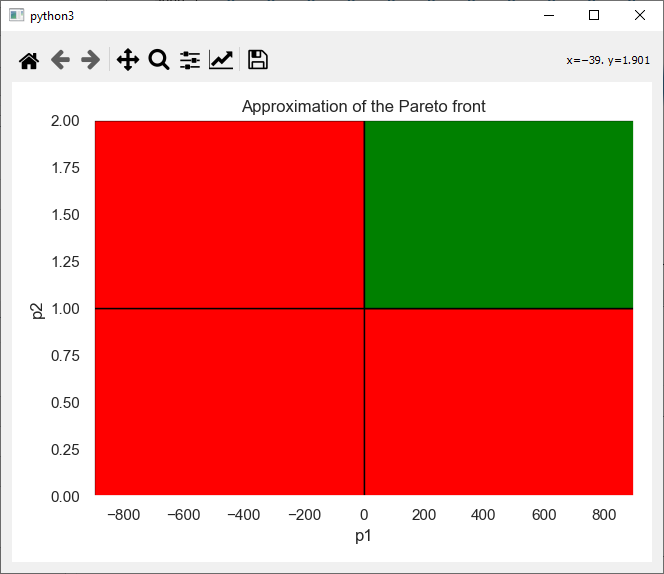
\includegraphics[width=0.7\linewidth]{images/stl_parametrico_der} 
\caption{Resultado paramétrico para la derivada.}
\label{fig:param_derivative}
\end{figure}


Asimismo, podemos ejecutar expresiones con integrales como por ejemplo:

$$On_{[0,p_1]} I\, \mathbf{x}_0 >= 5*10^6 - p_2$$ 

donde $p_1$ y $p_2$ son los parámetros, $\mathbf{x}_0$ es la señal, $I$ es el operador integral y $On_{[0,p_1]}$ indica el intervalo de integración.
Igualmente, ParetoLib devuelve como resultado la imagen \ref{fig:param_integral} que muestra las configuraciones de los parámetros $p_1$ y $p_2$ que satisfacen la propiedad (región en verde) y las que lo falsifican (región en rojo). 
Cabe mencionar que este tipo de mapas ya estaban previamente disponibles como resultado de la ejecución de la biblioteca de minería.

\begin{figure}[htb]
\centering
  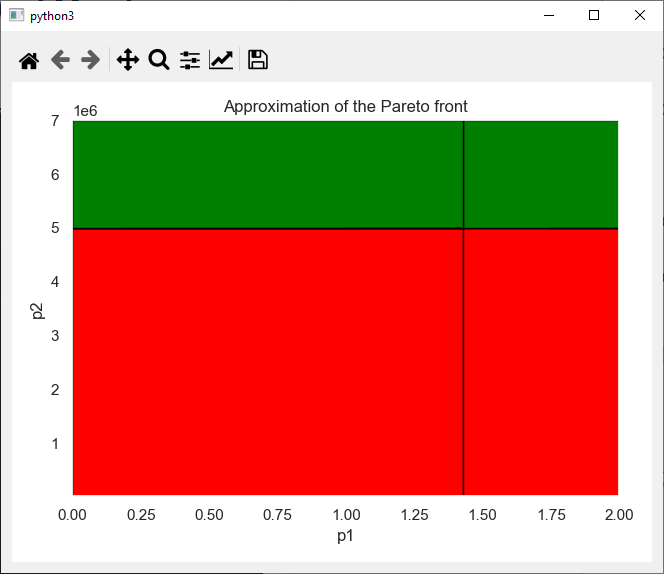
\includegraphics[width=0.7\linewidth]{images/stl_parametrico_int} 
\caption{Resultado paramétrico para la integral.}
\label{fig:param_integral}
\end{figure}

ParetoLib está escrito en Python. %La máquina virtual de Python, junto con los binarios y librerías de STLEval precompilados tanto para Linux como para Windows, convierten a ParetoLib en una biblioteca multiplataforma.
El código fuente \ref{list:paretolib_example} ilustra la forma tradicional de invocar a la biblioteca de minería. En el capitulo \ref{cha:gui} veremos la nueva interfaz gráfica que va a facilitar al usuario el trabajo con ParetoLib y con STLEval.

%\jicomment{TODO:
%\begin{itemize}
%\item Referenciar a la rama de ParetoLib/GUI donde se engloban los cambios de la GUI + los nuevos binarios de STLEval
%\item Describir un ejemplo de STL con parametros sobre un operador derivada/integral. Por ejemplo `` I [0, 20] sin(x) `` sería 0; ``F D sin(x) > 0`` sería True, ...
%\end{itemize}
%}

\lstinputlisting[language=python,
		style=python_style,
		label={list:paretolib_example},
		caption={Invocación de la biblioteca ParetoLib mediante código fuente en Python.}]
		{code/python/example2d_derivative.py}
